\documentclass{article}

% packages
\usepackage{amsmath, amsthm, thmtools, amsfonts, amssymb, luacode, catchfile, tikzducks, hyperref, ifthen}
\ifcsname c@kobocompile\endcsname
	\usepackage[a5paper, total={1072pt, 1448pt}, margin=10pt, includeheadfoot]{geometry} % set page margins
\else
	\usepackage[a4paper, margin=50pt, includeheadfoot]{geometry}
\fi
\usepackage[shortlabels]{enumitem}
\usepackage[skip=3pt, indent=0pt]{parskip}

% language
\usepackage[bidi=basic, layout=tabular, provide=*]{babel}
\ifcsname c@english\endcsname
	\babelprovide[main, import]{english}
\else
	\babelprovide[main, import]{hebrew}
	\babelprovide{rl}
\fi
%\babelfont{rm}{Libertinus Serif}
\babelfont{rm}[Renderer=Harfbuzz]{Libertinus Serif}
\babelfont{sf}{Libertinus Sans}
\babelfont{tt}{Libertinus Mono}

% style
\AddToHook{cmd/section/before}{\clearpage}	% Add line break before section
\linespread{1.3}
\setcounter{secnumdepth}{0}		% Remove default number tags from sections, this won't do well with theorems
\AtBeginDocument{\setlength{\belowdisplayskip}{3pt}}
\AtBeginDocument{\setlength{\abovedisplayskip}{3pt}}
\graphicspath{ {../images/} }

% operators
\DeclareMathOperator\cis{cis}
\DeclareMathOperator\Sp{Sp}
\DeclareMathOperator\tr{tr}
\DeclareMathOperator\im{Im}
\DeclareMathOperator\re{Re}
\DeclareMathOperator\diag{diag}
\DeclareMathOperator*\lowlim{\underline{lim}}
\DeclareMathOperator*\uplim{\overline{lim}}
\DeclareMathOperator\rng{rng}
\DeclareMathOperator\Sym{Sym}
\DeclareMathOperator\Arg{Arg}
\DeclareMathOperator\Log{Log}
\DeclareMathOperator\dom{dom}
\DeclareMathOperator\supp{Supp}
\DeclareMathOperator\var{Var}
\DeclareMathOperator\cov{Cov}

% commands
%\renewcommand\qedsymbol{\textbf{מש''ל}}
%\renewcommand\qedsymbol{\fbox{\emoji{lizard}}}
\newcommand{\Aa}[0]{\mathcal{A}}
\newcommand{\Bb}[0]{\mathcal{B}}
\newcommand{\CC}[0]{\mathbb{C}}
\newcommand{\Cc}[0]{\mathcal{C}}
\newcommand{\EE}[0]{\mathbb{E}}
\newcommand{\FF}[0]{\mathbb{F}}
\newcommand{\Ff}[0]{\mathcal{F}}
\newcommand{\Ii}[0]{\mathcal{I}}
\newcommand{\Gg}[0]{\mathcal{G}}
\newcommand{\Ll}[0]{\mathcal{L}}
\newcommand{\Mm}[0]{\mathcal{M}}
\newcommand{\NN}[0]{\mathbb{N}}
\newcommand{\Nn}[0]{\mathcal{N}}
\newcommand{\PP}[0]{\mathbb{P}}
\newcommand{\Pp}[0]{\mathcal{P}}
\newcommand{\QQ}[0]{\mathbb{Q}}
\newcommand{\RR}[0]{\mathbb{R}}
\newcommand{\Rr}[0]{\mathcal{R}}
\newcommand{\Ss}[0]{\mathcal{S}}
\newcommand{\TT}[0]{\mathbb{T}}
\newcommand{\Uu}[0]{\mathcal{U}}
\newcommand{\Vv}[0]{\mathcal{V}}
\newcommand{\Ww}[0]{\mathcal{W}}
\newcommand{\ZZ}[0]{\mathbb{Z}}
\newcommand{\acts}[0]{\circlearrowright}
\newcommand{\explain}[2] {
	\begin{flalign*}
		 && \text{#2} && \text{#1}
	\end{flalign*}
}
\newcommand{\maketitleprint}[0]{ \begin{center}
	%\begin{tikzpicture}[scale=3]
	%	\duck[graduate=gray!20!black, tassel=red!70!black]
	%\end{tikzpicture}	
	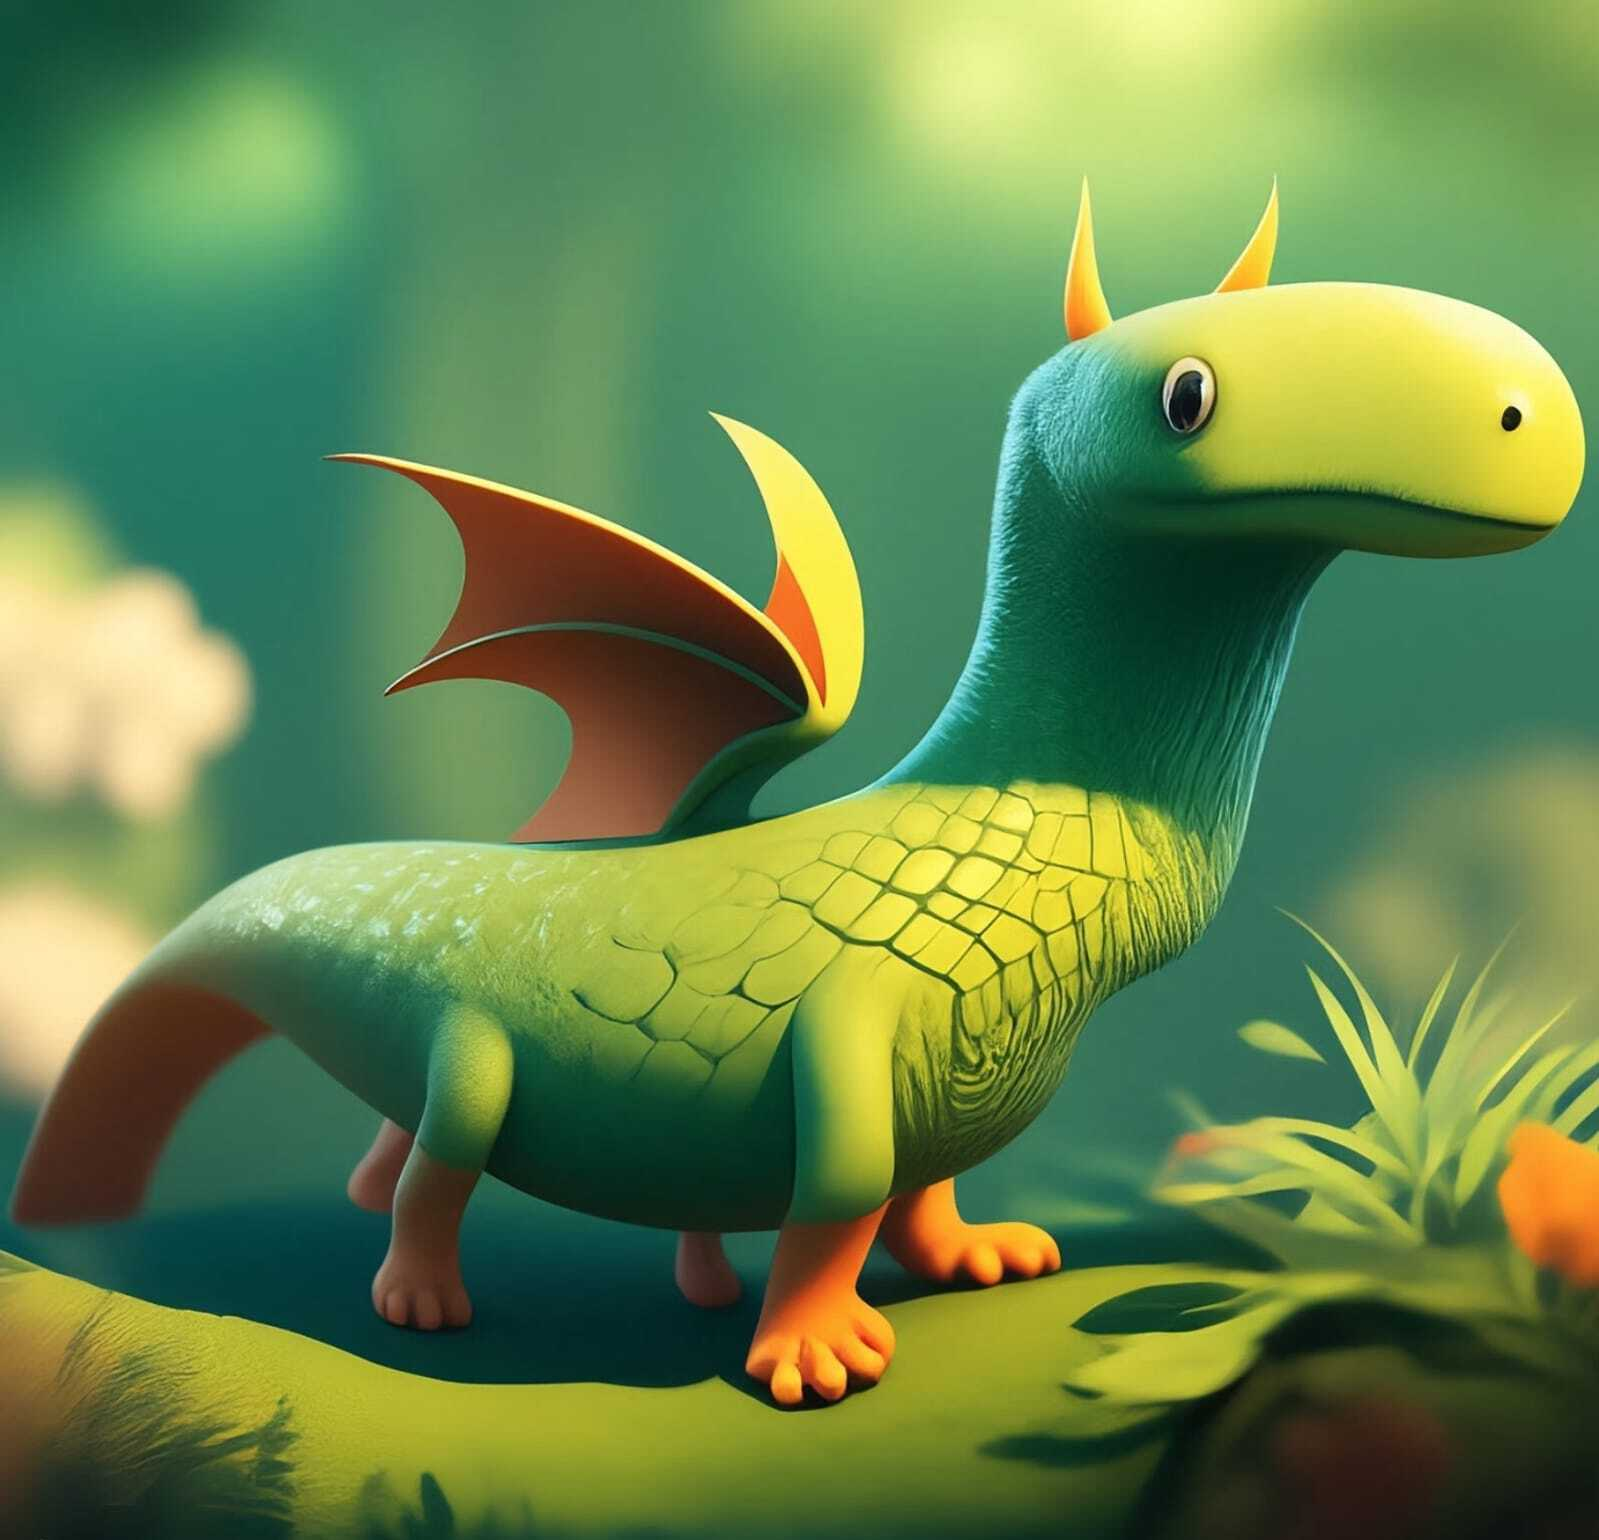
\includegraphics[width=6cm]{cover}
\end{center}
}

% theorem commands
\newtheoremstyle{c_remark}
	{}	% Space above
	{}	% Space below
	{}% Body font
	{}	% Indent amount
	{\bfseries}	% Theorem head font
	{}	% Punctuation after theorem head
	{.5em}	% Space after theorem head
	{\thmname{#1}\thmnumber{ #2}\thmnote{ \normalfont{\text{(#3)}}}}	% head content
\newtheoremstyle{c_definition}
	{3pt}	% Space above
	{3pt}	% Space below
	{}% Body font
	{}	% Indent amount
	{\bfseries}	% Theorem head font
	{}	% Punctuation after theorem head
	{.5em}	% Space after theorem head
	{\thmname{#1}\thmnumber{ #2}\thmnote{ \normalfont{\text{(#3)}}}}	% head content
\newtheoremstyle{c_plain}
	{3pt}	% Space above
	{3pt}	% Space below
	{\itshape}% Body font
	{}	% Indent amount
	{\bfseries}	% Theorem head font
	{}	% Punctuation after theorem head
	{.5em}	% Space after theorem head
	{\thmname{#1}\thmnumber{ #2}\thmnote{ \text{(#3)}}}	% head content

\ifcsname c@english\endcsname
	\theoremstyle{plain}
	\newtheorem{theorem}{Theorem}[section]
	\newtheorem{lemma}[theorem]{Lemma}
	\newtheorem{proposition}[theorem]{Proposition}
	\newtheorem*{proposition*}{Proposition}
	%\newtheorem{corollary}[theorem]{אין חלופה עברית}

	\theoremstyle{definition}
	\newtheorem{definition}[theorem]{Definition}
	\newtheorem*{definition*}{Definition}
	\newtheorem{example}{Example}[section]
	\newtheorem{exercise}{Exercise}[section]

	\theoremstyle{remark}
	\newtheorem*{remark}{Remark}
	\newtheorem*{solution}{Solution}
	\newtheorem{conclusion}[theorem]{Conclusion}
	\newtheorem{notation}[theorem]{Notation}
\else
	\theoremstyle{c_plain}
	\newtheorem{theorem}{משפט}[section]
	\newtheorem{lemma}[theorem]{למה}
	\newtheorem{proposition}[theorem]{טענה}
	\newtheorem*{proposition*}{טענה}
	%\newtheorem{corollary}[theorem]{אין חלופה עברית}

	\theoremstyle{c_definition}
	\newtheorem{definition}[theorem]{הגדרה}
	\newtheorem*{definition*}{הגדרה}
	\newtheorem{example}{דוגמה}[section]
	\newtheorem{exercise}{תרגיל}[section]

	\theoremstyle{c_remark}
	\newtheorem*{remark}{הערה}
	\newtheorem*{solution}{פתרון}
	\newtheorem{conclusion}[theorem]{מסקנה}
	\newtheorem{notation}[theorem]{סימון}
\fi

% Questions related commands
\newcounter{question}
\setcounter{question}{1}
\newcounter{sub_question}
\setcounter{sub_question}{1}

\ifcsname c@english\endcsname
	\newcommand{\question}[1][0]{
		\ifthenelse{#1 = 0}{}{\setcounter{question}{#1}}
		\section{Question \arabic{question}}
		\addtocounter{question}{1}
		\setcounter{sub_question}{1}
	}

	\newcommand{\subquestion}[1][0]{
		\ifthenelse{#1 = 0}{}{\setcounter{sub_question}{#1}}
		\subsection{Part \alph{sub_question}}
		\addtocounter{sub_question}{1}
	}
\else
	\newcommand{\question}[1][0]{
		\ifthenelse{#1 = 0}{}{\setcounter{question}{#1}}
		\section{שאלה \arabic{question}}
		\addtocounter{question}{1}
		\setcounter{sub_question}{1}
	}

	\newcommand{\subquestion}[1][0]{
		\ifthenelse{#1 = 0}{}{\setcounter{sub_question}{#1}}
		\subsection{סעיף \localecounter{letters.gershayim}{sub_question}}
		\addtocounter{sub_question}{1}
	}
\fi

% import lua and start of document
\directlua{common = require ('../common')}

\GetEnv{AUTHOR}

% headers
\author{\AUTHOR}
\date\today

\title{פתרון מטלה 02 --- מבנים אלגבריים (2), 80446}

\begin{document}
\maketitle
\maketitleprint{}

\question{}
יהי $K \subseteq \CC$ שדה שאינו מוכל ב־$\RR$. \\
נוכיח ש־$[K : K \cap \RR] = 2$.
\begin{proof}
	ממשפט האיזומורפיזם השני מתקיים $|(K + \RR) / \RR| = |K / (K \cap \RR)| = [K : K \cap \RR]$, אבל מתקיים $\CC = K + \RR$ מהנתון כי $K \subseteq \CC, \RR \not\subseteq K$, וכן $|\CC / \RR| = 2$ כפי שרצינו.
\end{proof}

\question{}
\subquestion{}
עבור $\alpha = \sqrt{3} + \sqrt{7} i \in \CC$ נמצא את $f_{\alpha / \QQ}(x)$, הפולינום המינימלי של $\alpha$ מעל $\QQ$.
\begin{solution}
	נבחין כי עבור $\sqrt{3}$ הפולינום המינימלי הוא $x^2 - 3$, זהו פולינום אי־פריק המחלק את הערך ולכן נוכל להסיק זאת, בנוסף מסיבות דומות גם $x^2 + 7$ פולינום מינימלי עבור $\sqrt{7}$.
	נובע אם כך ש־$\deg f_{\alpha / \QQ} \le 4$.
	עוד נבחין ש־$[\QQ[\sqrt{3}, \sqrt{7}i] : \QQ] = [\QQ[\sqrt{7}i] : \QQ] \cdot [\QQ[\sqrt{3}] : \QQ] = 4$, כלומר, דרגת הפולינום היא בדיוק $4$.
	בנוסף נבחין כי מתקיים,
	\begin{align*}
		& x - (\sqrt{3} + \sqrt{7} i) = 0 \\
		\iff & x - \sqrt{3} = \sqrt{7} i \\
		\iff & x^2 - 2 \sqrt{3} x + 3 = -7 \\
		\iff & x^4 + 20x^2 + 100 = 12x^2
	\end{align*}
	ולכן $f_{\alpha / \QQ} \mid x^4 + 8x^2 + 100$, אז נסיק ש־$f_{\alpha / \QQ}(x) = x^4 + 8x^2 + 100$ בדיוק.
\end{solution}

\subquestion{}
יהי $d \in \NN$ טבעי שאינו חזקה שלישית של מספר רציונלי, ויהיו $s, t \in \QQ$ שאינם שניהם אפס. \\
נסמן $\alpha = \sqrt[3]{d} \in \CC$ את אחד השורשים השלישיים של $d$.
עבור $\beta = s \alpha + t \alpha^2$ נבטא את הפולינום המינימלי $f_{\beta / \QQ}(x)$ של $\beta$ מעל $\QQ$ באמצעות $d, s, t$.
\begin{solution}
	כמו בסעיף הקודם, נוכל להסיק שדרגת הפולינום תהיה בדיוק $3$, ולכן נניח ש־$f = f_{\beta / \QQ}(x) = x^3 + c_2 x^2 + c_1 x + c_0$, ובהתאם $f(\beta) = 0$. \\
	נבחין שמתקיים,
	\[
		\beta^3
		= s^2 d + t^2 d^2 + 3(s^2 t \alpha^4 + s t^2 \alpha^5)
		= s^2 d + t^2 d^2 + 3std (s \alpha + t \alpha^2)
		= s^2 d + t^2 d^2 + 3std \beta
	\]
	ולכן הפולינום $f(x) = x^3 - 3std x - s^2 d - t^2 d^2$ מקיים $f(\beta) = 0$ וכן $\deg_\QQ f = 0$, ולכן הוא מקיים $f = f_{\beta / \QQ}$.
\end{solution}

\question{}
\subquestion{}
יהי $f \in \QQ[x]$ ונסמן $f(x) = a_n x^n + \cdots + a_1 x + a_0$.
נראה שאם $\frac{r}{s} \in \QQ$ שורש של $f$ אז $s \mid a_n, r \mid a_0$.
\begin{proof}
	נניח שהשבר $\frac{r}{s}$ הוא שבר מצומצם, לכן $r \nmid s$ וכן $s \nmid r$.
	נתחיל ונראה ש־$r \mid a_0$, נבחין כי, ידוע ש־$f(\frac{r}{s}) = 0$, לכן גם,
	\[
		0 = s^n f(\frac{r}{s})
		= a_n r^n + \cdots + a_1 r s^{n - 1} + a_0 s^n
	\]
	אבל בהתאם נקבל $a_0 s^n = -r(a_n r^{n - 1} + \cdots + a_1 s^{n - 1})$, ומההנחה על $s$ נקבל שגם $s^n \nmid r$, לכן $a_0 \mid r$.

	מהצד השני נקבל שגם $r^n a_n = -s (a_{n - 1} r^{n - 1} + \cdots + a_0 s^{n - 1})$, ולכן מאותה הסיבה נובע שגם $s \mid a_n$.
\end{proof}

\subquestion{}
נתאר שיטה המשתמשת במטלה 1 שאלה 4 ובסעיף א' של שאלה זו כדי לבדוק אם פולינום $f \in \QQ[x]$ כך ש־$\deg f \in \{2, 3\}$ הוא אי־פריק.
\begin{solution}
	במטלה 1 ראינו ש־$f$ אי־פריק אם ורק אם $f(\alpha) \ne 0$ לכל $\alpha \in \QQ$.
	נניח גם ש־$f$ מתוקן, ולכן נובע שאם $\alpha = \frac{r}{s}$ אז $s \mid a_n$, כלומר $\alpha \in \ZZ$.
	אבל אנו גם יודעים ש־$\alpha \mid a_0$, ולכן מספיק לבדוק את המחלקים של $a_0$ בלבד.
\end{solution}

\subsubsection{i}
נבדוק את $f(x) = x^3 - 4x + 2$.
\begin{solution}
	נבחין כי אכן הפולינום מתוקן, ולכן מספיק לבדוק את $\pm 1, \pm 2$ בלבד, ונבחין כי אכן $f(\pm1) = \pm1 \mp 4 + 2 \ne 0$ וכן ש־$f(\pm2) = \pm 8 \mp 8 + 2 \ne 0$, לכן הפולינום אי־פריק.
\end{solution}

\subsubsection{ii}
נבדוק את $f(x) = x^3 - 4x^2 + 3x + 3$.
\begin{solution}
	גם הפעם מספיק שנבדוק את $1, 3$ בלבד, ונבחין כי $f(\pm1) = \pm 1 - 4 \pm 3 + 3 \ne 0$ וכן $f(\pm3) = \pm 27 - 36 \pm 9 + 3 \ne 0$ ולכן גם הפולינום הזה אי־פריק.
\end{solution}

\question{}
תהי $E / F$ הרחבת שדות, ויהי $f \in F[x]$ אי־פריק כך ש־$L = F[x] / (f)$.
נסמן ב־$\alpha$ את התמונה של $x$ ב־$L$, כלומר $\alpha = x + (f)$.
נניח ש־$\varphi : L \to E$ הוא $F$־הומומורפיזם.

\subquestion{}
נראה ש־$\varphi(\alpha) \in E$ הוא שורש של $f \in F[x] \subseteq E[x]$.
\begin{proof}
	אנו רוצים להראות ש־$f(\varphi(\alpha)) = 0$.
	נבחין תחילה שפולינומים הם הרכבה של חיבור ומכפלה, ולכן נובע ישירות שמתקיים,
	\[
		f(\varphi(\alpha)) = \varphi(f(\alpha)) = \varphi(0 + f(x)) = 0
	\]
	כאשר המעבר האחרון נובע משימור האיבר הנייטרלי לחיבור.
\end{proof}

\subquestion{}
נוכיח שאם $\psi : L \to E$ הוא $F$־הומומורפיזם נוסף כך ש־$\varphi(\alpha) = \psi(\alpha)$ אז $\varphi = \psi$.
\begin{proof}
	נבחין כי $\varphi \restriction F = \psi \restriction F$, ולכן עלינו רק לבדוק זהות בערכים $L \setminus F$.
	אנו גם יודעים ש־$\alpha, \ldots, \alpha^{n - 1}$ עבור $n = \deg_F f$ בסיס של $L$ מעל $F$, לכן עלינו לבדוק ערכים אלה בלבד.
	אבל נתון ש־$\varphi(\alpha^k) = {\varphi(\alpha)}^k = {\psi(\alpha)}^k = \psi(\alpha^k)$, ולכן נוכל להסיק ש־$\varphi = \psi$.
\end{proof}

\question{}
בשאלה זו ננסה ונבנה הרחבה $E / \QQ$ כך ש־$[E : \QQ] = 3$ אבל אין $d \in \QQ$ כך ש־$E \simeq \QQ(\sqrt[3]{d})$.

\subquestion{}
יהי $d \in \QQ$ שאינו חזקה שלישית של מספר רציונלי, נראה שקיים הומומורפיזם  $\varphi : \QQ(\sqrt[3]{d}) \to \CC$ כך ש־$\im \varphi \not\subseteq \RR$.
\begin{proof}
	מטרתנו היא למפות את השורשים לשורשים מרוכבים.
	כלומר נגדיר את $\varphi(\sqrt[3]{d^k}) = |\sqrt[3]{d^k}| \exp(\frac{2\pi i + 2\pi k}{3})$ עבור $k \in \{0, 1, 2\}$, וכן $\varphi(q) = q$ עבור $q \in \QQ$.
	עלינו להראות כי זהו אכן הומומורפיזם.
	עבור $\QQ$ קיום התכונה הוא ישיר מהגדרה.
	עבור כפל של רציונלי בשורש ישיר, ולכן מספיק שנבדוק את המקרה של כפל שורשים.
	מההגדרה מתקיים $\varphi(\sqrt[3]{d}) \cdot \varphi(\sqrt[3]{d}) = \varphi(\sqrt[3]{d^2})$, וכן מתקיים,
	\[
		\varphi(\sqrt[3]{d}) \cdot \varphi(\sqrt[3]{d^2})
		= |\sqrt[3]{d}| \exp(\frac{2\pi i}{3}) \cdot |\sqrt[3]{d^2}| \exp(\frac{2\pi i + 2\pi}{3})
		= d
	\]
	ולכן $\varphi$ אכן הומומורפיזם.
\end{proof}

\subquestion{}
יהי $f \in \QQ[x]$ אי־פריק מדרגה 3 כך ששלושת השורשים של $f$ ממשיים ואי־רציונליים.
נראה ש־$L = \QQ[x] / (f)$ שדה כך ש־$[L : \QQ] = 3$, ושאם $\varphi : L \to \CC$ הומומורפיזם, אז $\im \varphi \subseteq \RR$.
\begin{proof}
	אנו יודעים ש־$(f)$ אידאל ראשי וכן ש־$L$ שדה.
	אנו גם יודעים ש־$f$ מהווה פולינום מינימלי ולכן $[L : \QQ] = 3$. \\
	יהי $\varphi : L \to \CC$ הומומורפיזם.
	ידוע ש־$\varphi(1) = 1$ ולכן $\varphi(\QQ) \subseteq \RR$, ומספיק שנבדוק את התמונה של $\alpha_1, \alpha_2, \alpha_3$ השורשים של $f$.
	נתון כי $\alpha_i \in \RR \setminus \QQ$ לכל $i \in [3]$, וכן ידוע ש־$L \simeq \QQ[\{ \alpha_i \}]$, ולכן מהרכבת איזומורפיזמים ומשפט האיזומורפיזם הראשון נסיק ש־$\varphi(\alpha_i) = \alpha_i \in \RR$ בלבד.
\end{proof}

\subquestion{}
נוכיח ש־$f(x) = x^3 - 4x + 2$ פולינום המקיים את תנאי סעיף ב', ונסיק ש־$E = \QQ[x] / (f)$ הרחבה מסדר 3 של $\QQ$ שאינה איזומורפית לשדה מהצורה $\QQ(\sqrt[3]{d})$.
\begin{proof}
	בשאלה 3 ראינו כבר כי $f$ פולינום אי־פריק, הוא אכן מדרגה 3, ולכן עלינו רק להראות ששורשיו לא רציונליים.
	נבחין כי $f'(x) = 3x^2 - 4$, ולכן ל־$f$ נקודות קיצון ב־$x = \sqrt{\frac{4}{3}}$, ולכן נבדוק ונקבל שמתקיים,
	\[
		f(-3) = -13,
		f(0) = 2,
		f(1) = -1,
		f(2) = 2
	\]
	כלומר, מצאנו שתי נקודות שבינן ישנו שורש של הפונקציה, עתה ממשפט ערך הביניים נסיק כי קיימים שלושה שורשים בתחומים אלה, כלומר ישנם שלושה שורשים ממשיים.
	אנו גם יודעים כי הפולינום הוא לא פריק מעל הרציונליים, לכן שורשים אלה לא רציונליים.
	בהתאם כל תנאי סעיף ב' חלים ולכל הומומורפיזם $\varphi : \QQ[x] / (f) \to \CC$ מתקיים $\im \varphi \subseteq \CC$.
	אילו נניח בשלילה שקיים $d \in \QQ$ כך ש־$\QQ[x] / (f) \simeq \QQ(\sqrt[3]{d})$, אז נקבל מההומומורפיזם שבנינו בסעיף א' סתירה, שכן $\varphi \subseteq \RR$ אבל $\varphi \not\subseteq \RR$, לכן אין $d$ כזה.
\end{proof}

\end{document}
